% Sección 3 (EDA), continuación de las subsecciones de P1 (fuente, selección de
% estación y periodo). Se inserta con % Sección 3 (EDA), continuación de las subsecciones de P1 (fuente, selección de
% estación y periodo). Se inserta con % Sección 3 (EDA), continuación de las subsecciones de P1 (fuente, selección de
% estación y periodo). Se inserta con % Sección 3 (EDA), continuación de las subsecciones de P1 (fuente, selección de
% estación y periodo). Se inserta con \input{seccion_3_eda} después de ellas.
% Figuras esperadas en figures/ (las mismas de la notebook 01_eda).

\subsection{Calidad de los datos y valores faltantes}
\label{sec:faltantes}

De las 20.424 horas del periodo, 1.033 (5,06~\%) no tienen medición de PM2.5. Esa cifra agregada describe mal el problema: las ausencias se agrupan en 47 interrupciones con una mediana de 11 horas, y las 12 que duran 24 horas o más concentran 700 horas, el 68~\% de todos los faltantes (la mayor dura 126 horas). El archivo no documenta la causa, por lo que no puede asumirse que los faltantes sean aleatorios. Si coincidieran con episodios de alta concentración, los estadísticos descriptivos subestimarían los valores extremos. Por eso no se imputa ni se interpola ningún valor: las horas sin medición se conservan explícitamente en la serie.

Se aplicaron tres controles de coherencia. Ninguna de las 18.671 horas con PM2.5 y PM10 simultáneos presenta PM2.5 por encima de PM10, la racha máxima de valores idénticos consecutivos es de 2 (descarta un sensor bloqueado) y se observaron 49 variaciones horarias superiores a 50~\textmu g/m\textsuperscript{3}, con un máximo de 121,0. Estas últimas se señalan para revisión, pero no se descartan.

\subsection{Distribución y valores extremos}
\label{sec:distribucion}

La serie disponible (19.391 mediciones) tiene media de 29,29 y mediana de 24,50~\textmu g/m\textsuperscript{3}, desviación estándar de 18,17, percentil 95 de 65,31 y máximo de 191,5. La asimetría es de 2,11: una minoría de horas con concentraciones altas arrastra el promedio. Al ser la variable objetivo continua, no existe un desbalance de clases en sentido estricto, pero la distribución produce un efecto equivalente, porque las concentraciones altas están poco representadas.

La regla de 1,5 veces el rango intercuartílico señala 1.126 mediciones (5,81~\%). No se eliminan: el 95~\% corresponde a 2022, se concentran entre mayo y octubre y entre las 12:00 y las 16:00, que es la franja de mayor mediana horaria. Un error instrumental no reproduciría esa estructura estacional y horaria, de modo que la evidencia favorece interpretarlas como episodios reales de contaminación, que además son las horas de mayor relevancia sanitaria. Como contexto, de los 795 días con al menos 18 horas medidas, el 93~\% supera la guía diaria de la OMS (15~\textmu g/m\textsuperscript{3}) y el 10,3~\% el estándar peruano (50~\textmu g/m\textsuperscript{3}).

\subsection{Patrón diario y cambio de régimen}
\label{sec:regimen}

La mediana horaria alcanza su máximo a las 14:00 (34,4~\textmu g/m\textsuperscript{3}) y su mínimo a las 22:00 (17,0), por lo que la hora del día está asociada al nivel de PM2.5. Esta es una diferencia descriptiva; que mejore la predicción debe comprobarse con modelos.

El nivel medio desciende a lo largo del periodo: 38,8~\textmu g/m\textsuperscript{3} en 2022, 23,8 en 2023 y 17,7 en enero–abril de 2024. Parte de la caída de 2024 es estacional, pero 2022 supera a 2023 en 11 de los 12 meses, con una diferencia concentrada entre mayo y octubre, de modo que el calendario no la explica por completo (Fig.~\ref{fig:regimen}). Una partición cronológica entrena entonces en un régimen de concentraciones más altas que el de evaluación, y el error absoluto no es comparable entre tramos; las métricas deberán reportarse por separado para cada bloque.

\begin{figure}[t]
\centering
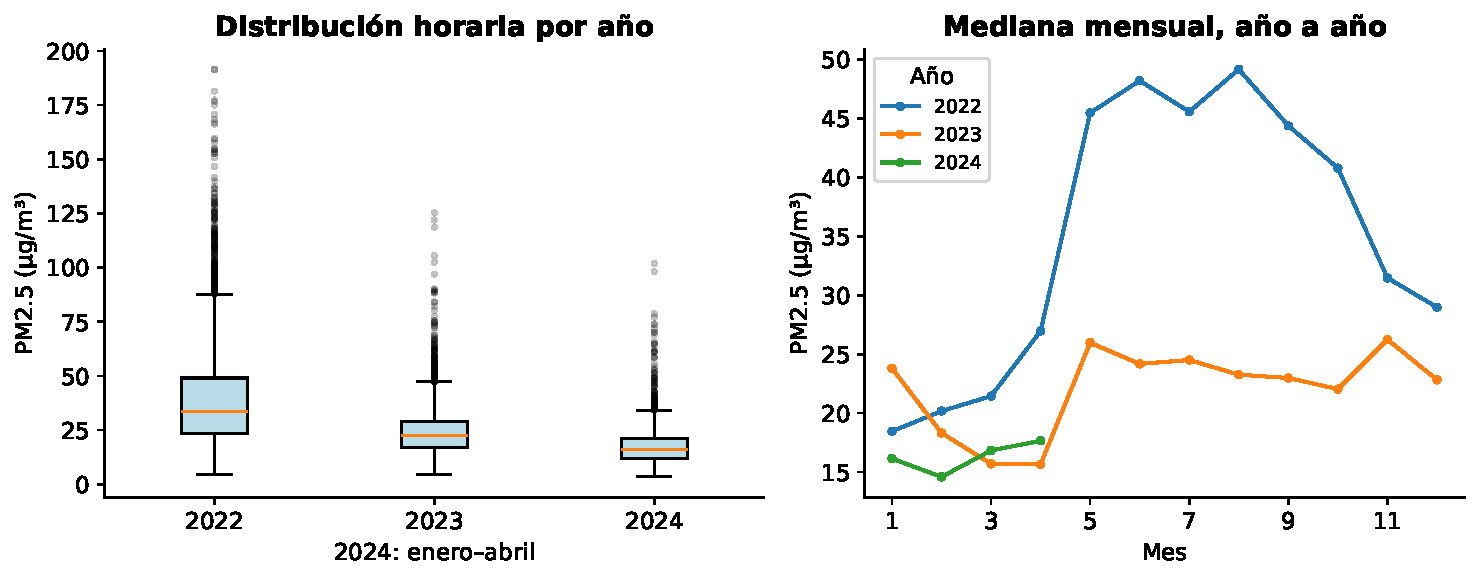
\includegraphics[width=\columnwidth]{figures/12_distribucion_anual.pdf}
\caption{Cambio de nivel entre años y comparación de medianas mensuales.}
\label{fig:regimen}
\end{figure}

\subsection{Dependencia temporal}
\label{sec:autocorrelacion}

Entre horas consecutivas la correlación de Pearson es de 0,912 (19.343 pares completos). La autocorrelación cae a 0,464 en el rezago 12 y vuelve a subir a 0,651 en el rezago 24, lo que muestra el ciclo diario. La autocorrelación parcial se concentra en el primer rezago (0,912), es negativa en el segundo ($-0{,}184$) y no supera 0,12 en valor absoluto entre los rezagos 3 y 24 (Fig.~\ref{fig:acf}). Los rezagos inmediatos aportan la información propia de corto plazo, mientras que el repunte a 24 horas corresponde al ciclo diario y puede representarse con variables de calendario en lugar de decenas de rezagos. Cuál de las dos opciones rinde más se responde comparando modelos con y sin calendario (pregunta de investigación 2).

\begin{figure}[t]
\centering
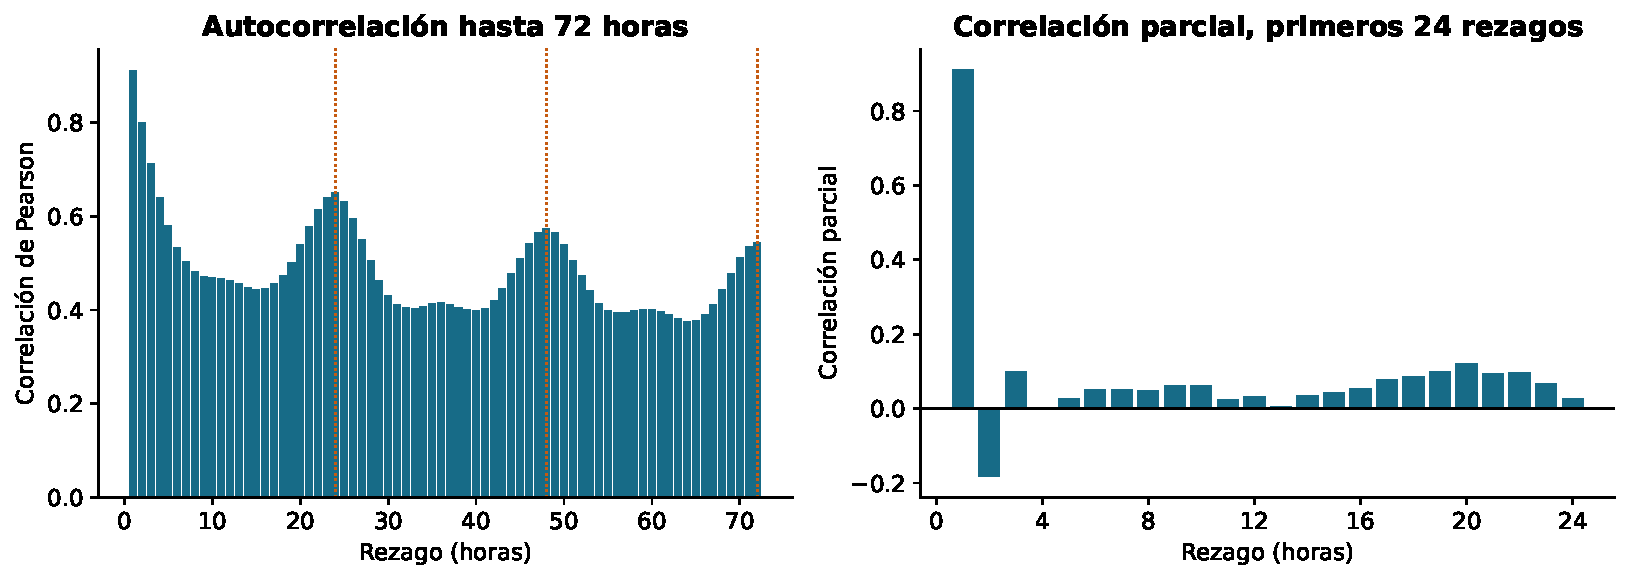
\includegraphics[width=\columnwidth]{figures/13_autocorrelacion.pdf}
\caption{Autocorrelación y autocorrelación parcial de PM2.5 hasta 48 horas, calculadas con las horas en que ambos valores están disponibles.}
\label{fig:acf}
\end{figure}

\subsection{Implicaciones para el modelado}
\label{sec:implicaciones}

El análisis exploratorio condiciona el diseño de la segunda etapa en cuatro puntos: los faltantes se agrupan en tramos y no se imputan, por lo que cada hora utilizable exige respuesta e historial completos; los valores extremos se conservan; la partición debe ser cronológica y sus métricas desagregadas por bloque, por el cambio de régimen; y el baseline natural es la persistencia, dada la correlación de 0,912 a una hora. Estas decisiones se concretan en la sección~\ref{sec:preproc}.
 después de ellas.
% Figuras esperadas en figures/ (las mismas de la notebook 01_eda).

\subsection{Calidad de los datos y valores faltantes}
\label{sec:faltantes}

De las 20.424 horas del periodo, 1.033 (5,06~\%) no tienen medición de PM2.5. Esa cifra agregada describe mal el problema: las ausencias se agrupan en 47 interrupciones con una mediana de 11 horas, y las 12 que duran 24 horas o más concentran 700 horas, el 68~\% de todos los faltantes (la mayor dura 126 horas). El archivo no documenta la causa, por lo que no puede asumirse que los faltantes sean aleatorios. Si coincidieran con episodios de alta concentración, los estadísticos descriptivos subestimarían los valores extremos. Por eso no se imputa ni se interpola ningún valor: las horas sin medición se conservan explícitamente en la serie.

Se aplicaron tres controles de coherencia. Ninguna de las 18.671 horas con PM2.5 y PM10 simultáneos presenta PM2.5 por encima de PM10, la racha máxima de valores idénticos consecutivos es de 2 (descarta un sensor bloqueado) y se observaron 49 variaciones horarias superiores a 50~\textmu g/m\textsuperscript{3}, con un máximo de 121,0. Estas últimas se señalan para revisión, pero no se descartan.

\subsection{Distribución y valores extremos}
\label{sec:distribucion}

La serie disponible (19.391 mediciones) tiene media de 29,29 y mediana de 24,50~\textmu g/m\textsuperscript{3}, desviación estándar de 18,17, percentil 95 de 65,31 y máximo de 191,5. La asimetría es de 2,11: una minoría de horas con concentraciones altas arrastra el promedio. Al ser la variable objetivo continua, no existe un desbalance de clases en sentido estricto, pero la distribución produce un efecto equivalente, porque las concentraciones altas están poco representadas.

La regla de 1,5 veces el rango intercuartílico señala 1.126 mediciones (5,81~\%). No se eliminan: el 95~\% corresponde a 2022, se concentran entre mayo y octubre y entre las 12:00 y las 16:00, que es la franja de mayor mediana horaria. Un error instrumental no reproduciría esa estructura estacional y horaria, de modo que la evidencia favorece interpretarlas como episodios reales de contaminación, que además son las horas de mayor relevancia sanitaria. Como contexto, de los 795 días con al menos 18 horas medidas, el 93~\% supera la guía diaria de la OMS (15~\textmu g/m\textsuperscript{3}) y el 10,3~\% el estándar peruano (50~\textmu g/m\textsuperscript{3}).

\subsection{Patrón diario y cambio de régimen}
\label{sec:regimen}

La mediana horaria alcanza su máximo a las 14:00 (34,4~\textmu g/m\textsuperscript{3}) y su mínimo a las 22:00 (17,0), por lo que la hora del día está asociada al nivel de PM2.5. Esta es una diferencia descriptiva; que mejore la predicción debe comprobarse con modelos.

El nivel medio desciende a lo largo del periodo: 38,8~\textmu g/m\textsuperscript{3} en 2022, 23,8 en 2023 y 17,7 en enero–abril de 2024. Parte de la caída de 2024 es estacional, pero 2022 supera a 2023 en 11 de los 12 meses, con una diferencia concentrada entre mayo y octubre, de modo que el calendario no la explica por completo (Fig.~\ref{fig:regimen}). Una partición cronológica entrena entonces en un régimen de concentraciones más altas que el de evaluación, y el error absoluto no es comparable entre tramos; las métricas deberán reportarse por separado para cada bloque.

\begin{figure}[t]
\centering
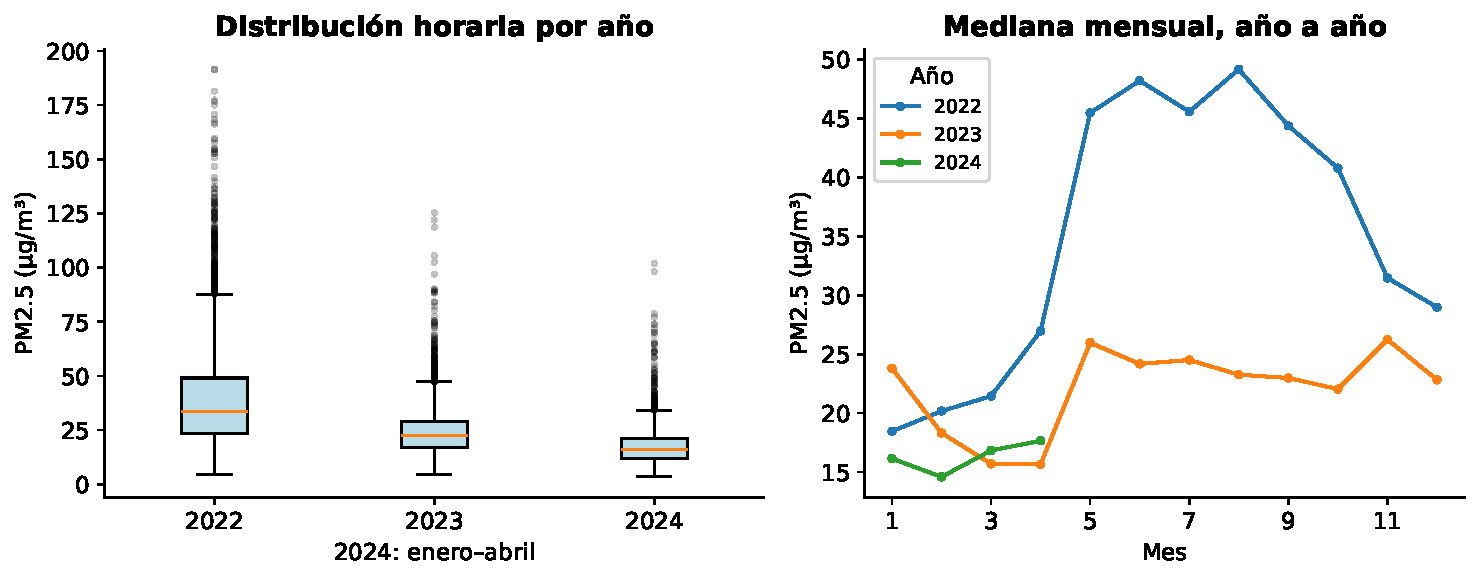
\includegraphics[width=\columnwidth]{figures/12_distribucion_anual.pdf}
\caption{Cambio de nivel entre años y comparación de medianas mensuales.}
\label{fig:regimen}
\end{figure}

\subsection{Dependencia temporal}
\label{sec:autocorrelacion}

Entre horas consecutivas la correlación de Pearson es de 0,912 (19.343 pares completos). La autocorrelación cae a 0,464 en el rezago 12 y vuelve a subir a 0,651 en el rezago 24, lo que muestra el ciclo diario. La autocorrelación parcial se concentra en el primer rezago (0,912), es negativa en el segundo ($-0{,}184$) y no supera 0,12 en valor absoluto entre los rezagos 3 y 24 (Fig.~\ref{fig:acf}). Los rezagos inmediatos aportan la información propia de corto plazo, mientras que el repunte a 24 horas corresponde al ciclo diario y puede representarse con variables de calendario en lugar de decenas de rezagos. Cuál de las dos opciones rinde más se responde comparando modelos con y sin calendario (pregunta de investigación 2).

\begin{figure}[t]
\centering
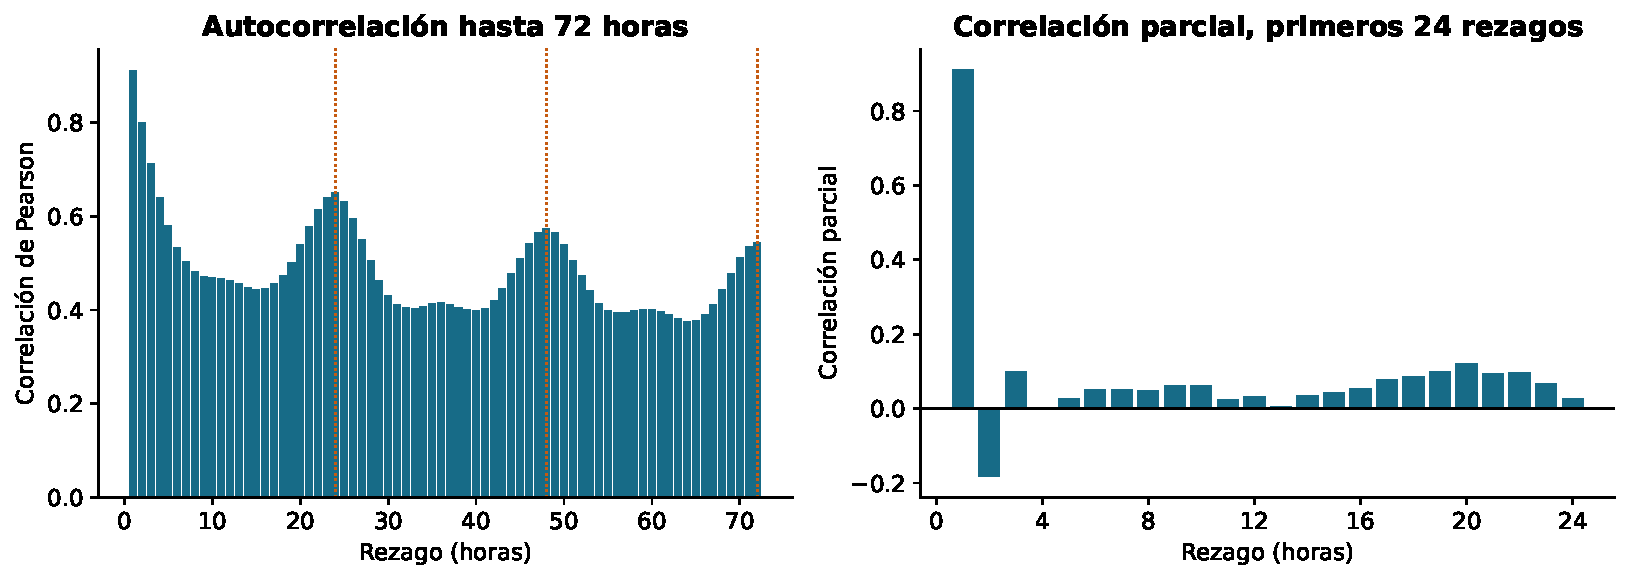
\includegraphics[width=\columnwidth]{figures/13_autocorrelacion.pdf}
\caption{Autocorrelación y autocorrelación parcial de PM2.5 hasta 48 horas, calculadas con las horas en que ambos valores están disponibles.}
\label{fig:acf}
\end{figure}

\subsection{Implicaciones para el modelado}
\label{sec:implicaciones}

El análisis exploratorio condiciona el diseño de la segunda etapa en cuatro puntos: los faltantes se agrupan en tramos y no se imputan, por lo que cada hora utilizable exige respuesta e historial completos; los valores extremos se conservan; la partición debe ser cronológica y sus métricas desagregadas por bloque, por el cambio de régimen; y el baseline natural es la persistencia, dada la correlación de 0,912 a una hora. Estas decisiones se concretan en la sección~\ref{sec:preproc}.
 después de ellas.
% Figuras esperadas en figures/ (las mismas de la notebook 01_eda).

\subsection{Calidad de los datos y valores faltantes}
\label{sec:faltantes}

De las 20.424 horas del periodo, 1.033 (5,06~\%) no tienen medición de PM2.5. Esa cifra agregada describe mal el problema: las ausencias se agrupan en 47 interrupciones con una mediana de 11 horas, y las 12 que duran 24 horas o más concentran 700 horas, el 68~\% de todos los faltantes (la mayor dura 126 horas). El archivo no documenta la causa, por lo que no puede asumirse que los faltantes sean aleatorios. Si coincidieran con episodios de alta concentración, los estadísticos descriptivos subestimarían los valores extremos. Por eso no se imputa ni se interpola ningún valor: las horas sin medición se conservan explícitamente en la serie.

Se aplicaron tres controles de coherencia. Ninguna de las 18.671 horas con PM2.5 y PM10 simultáneos presenta PM2.5 por encima de PM10, la racha máxima de valores idénticos consecutivos es de 2 (descarta un sensor bloqueado) y se observaron 49 variaciones horarias superiores a 50~\textmu g/m\textsuperscript{3}, con un máximo de 121,0. Estas últimas se señalan para revisión, pero no se descartan.

\subsection{Distribución y valores extremos}
\label{sec:distribucion}

La serie disponible (19.391 mediciones) tiene media de 29,29 y mediana de 24,50~\textmu g/m\textsuperscript{3}, desviación estándar de 18,17, percentil 95 de 65,31 y máximo de 191,5. La asimetría es de 2,11: una minoría de horas con concentraciones altas arrastra el promedio. Al ser la variable objetivo continua, no existe un desbalance de clases en sentido estricto, pero la distribución produce un efecto equivalente, porque las concentraciones altas están poco representadas.

La regla de 1,5 veces el rango intercuartílico señala 1.126 mediciones (5,81~\%). No se eliminan: el 95~\% corresponde a 2022, se concentran entre mayo y octubre y entre las 12:00 y las 16:00, que es la franja de mayor mediana horaria. Un error instrumental no reproduciría esa estructura estacional y horaria, de modo que la evidencia favorece interpretarlas como episodios reales de contaminación, que además son las horas de mayor relevancia sanitaria. Como contexto, de los 795 días con al menos 18 horas medidas, el 93~\% supera la guía diaria de la OMS (15~\textmu g/m\textsuperscript{3}) y el 10,3~\% el estándar peruano (50~\textmu g/m\textsuperscript{3}).

\subsection{Patrón diario y cambio de régimen}
\label{sec:regimen}

La mediana horaria alcanza su máximo a las 14:00 (34,4~\textmu g/m\textsuperscript{3}) y su mínimo a las 22:00 (17,0), por lo que la hora del día está asociada al nivel de PM2.5. Esta es una diferencia descriptiva; que mejore la predicción debe comprobarse con modelos.

El nivel medio desciende a lo largo del periodo: 38,8~\textmu g/m\textsuperscript{3} en 2022, 23,8 en 2023 y 17,7 en enero–abril de 2024. Parte de la caída de 2024 es estacional, pero 2022 supera a 2023 en 11 de los 12 meses, con una diferencia concentrada entre mayo y octubre, de modo que el calendario no la explica por completo (Fig.~\ref{fig:regimen}). Una partición cronológica entrena entonces en un régimen de concentraciones más altas que el de evaluación, y el error absoluto no es comparable entre tramos; las métricas deberán reportarse por separado para cada bloque.

\begin{figure}[t]
\centering
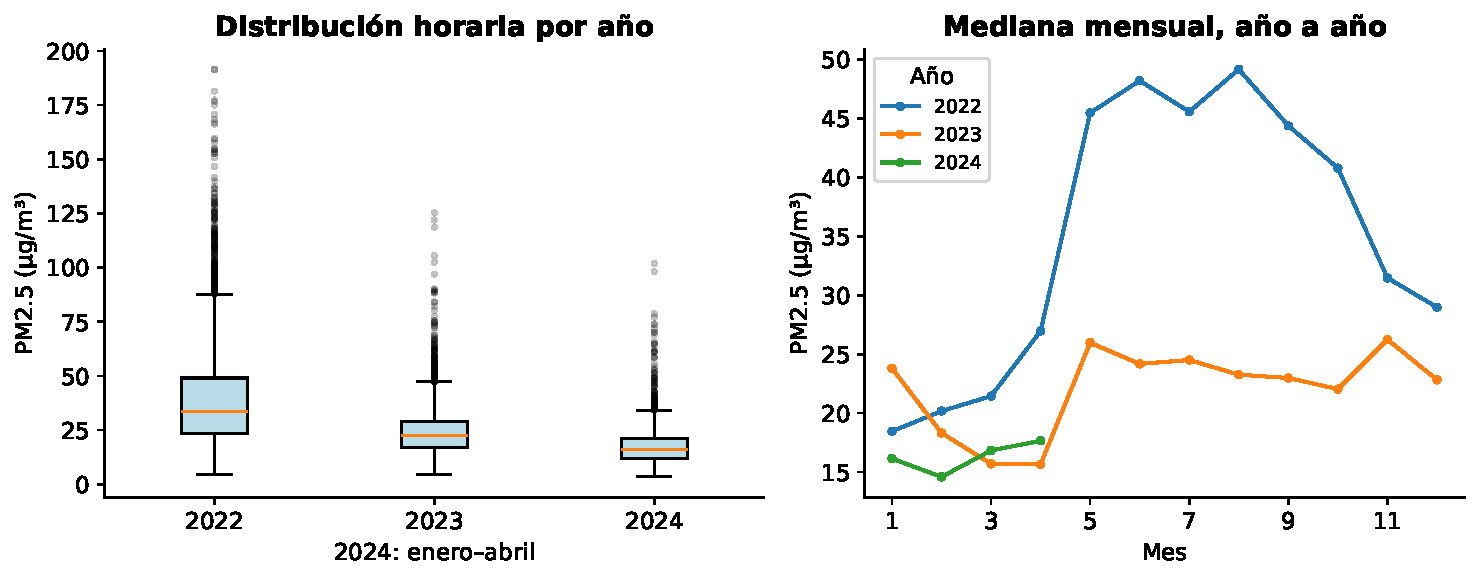
\includegraphics[width=\columnwidth]{figures/12_distribucion_anual.pdf}
\caption{Cambio de nivel entre años y comparación de medianas mensuales.}
\label{fig:regimen}
\end{figure}

\subsection{Dependencia temporal}
\label{sec:autocorrelacion}

Entre horas consecutivas la correlación de Pearson es de 0,912 (19.343 pares completos). La autocorrelación cae a 0,464 en el rezago 12 y vuelve a subir a 0,651 en el rezago 24, lo que muestra el ciclo diario. La autocorrelación parcial se concentra en el primer rezago (0,912), es negativa en el segundo ($-0{,}184$) y no supera 0,12 en valor absoluto entre los rezagos 3 y 24 (Fig.~\ref{fig:acf}). Los rezagos inmediatos aportan la información propia de corto plazo, mientras que el repunte a 24 horas corresponde al ciclo diario y puede representarse con variables de calendario en lugar de decenas de rezagos. Cuál de las dos opciones rinde más se responde comparando modelos con y sin calendario (pregunta de investigación 2).

\begin{figure}[t]
\centering
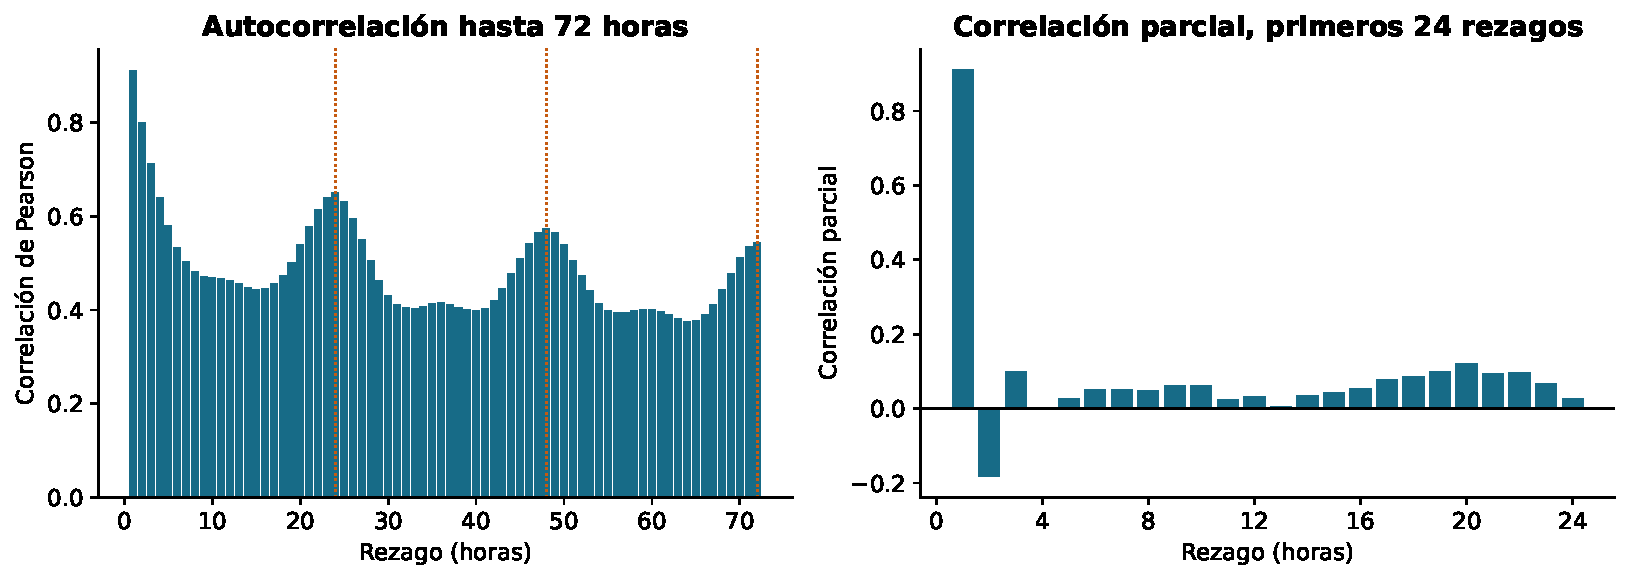
\includegraphics[width=\columnwidth]{figures/13_autocorrelacion.pdf}
\caption{Autocorrelación y autocorrelación parcial de PM2.5 hasta 48 horas, calculadas con las horas en que ambos valores están disponibles.}
\label{fig:acf}
\end{figure}

\subsection{Implicaciones para el modelado}
\label{sec:implicaciones}

El análisis exploratorio condiciona el diseño de la segunda etapa en cuatro puntos: los faltantes se agrupan en tramos y no se imputan, por lo que cada hora utilizable exige respuesta e historial completos; los valores extremos se conservan; la partición debe ser cronológica y sus métricas desagregadas por bloque, por el cambio de régimen; y el baseline natural es la persistencia, dada la correlación de 0,912 a una hora. Estas decisiones se concretan en la sección~\ref{sec:preproc}.
 después de ellas.
% Figuras esperadas en figures/ (las mismas de la notebook 01_eda).

\subsection{Calidad de los datos y valores faltantes}
\label{sec:faltantes}

De las 20.424 horas del periodo, 1.033 (5,06~\%) no tienen medición de PM2.5. Esa cifra agregada describe mal el problema: las ausencias se agrupan en 47 interrupciones con una mediana de 11 horas, y las 12 que duran 24 horas o más concentran 700 horas, el 68~\% de todos los faltantes (la mayor dura 126 horas). El archivo no documenta la causa, por lo que no puede asumirse que los faltantes sean aleatorios. Si coincidieran con episodios de alta concentración, los estadísticos descriptivos subestimarían los valores extremos. Por eso no se imputa ni se interpola ningún valor: las horas sin medición se conservan explícitamente en la serie.

Se aplicaron tres controles de coherencia. Ninguna de las 18.671 horas con PM2.5 y PM10 simultáneos presenta PM2.5 por encima de PM10, la racha máxima de valores idénticos consecutivos es de 2 (descarta un sensor bloqueado) y se observaron 49 variaciones horarias superiores a 50~\textmu g/m\textsuperscript{3}, con un máximo de 121,0. Estas últimas se señalan para revisión, pero no se descartan.

\subsection{Distribución y valores extremos}
\label{sec:distribucion}

La serie disponible (19.391 mediciones) tiene media de 29,29 y mediana de 24,50~\textmu g/m\textsuperscript{3}, desviación estándar de 18,17, percentil 95 de 65,31 y máximo de 191,5. La asimetría es de 2,11: una minoría de horas con concentraciones altas arrastra el promedio. Al ser la variable objetivo continua, no existe un desbalance de clases en sentido estricto, pero la distribución produce un efecto equivalente, porque las concentraciones altas están poco representadas.

La regla de 1,5 veces el rango intercuartílico señala 1.126 mediciones (5,81~\%). No se eliminan: el 95~\% corresponde a 2022, se concentran entre mayo y octubre y entre las 12:00 y las 16:00, que es la franja de mayor mediana horaria. Un error instrumental no reproduciría esa estructura estacional y horaria, de modo que la evidencia favorece interpretarlas como episodios reales de contaminación, que además son las horas de mayor relevancia sanitaria. Como contexto, de los 795 días con al menos 18 horas medidas, el 93~\% supera la guía diaria de la OMS (15~\textmu g/m\textsuperscript{3}) y el 10,3~\% el estándar peruano (50~\textmu g/m\textsuperscript{3}).

\subsection{Patrón diario y cambio de régimen}
\label{sec:regimen}

La mediana horaria alcanza su máximo a las 14:00 (34,4~\textmu g/m\textsuperscript{3}) y su mínimo a las 22:00 (17,0), por lo que la hora del día está asociada al nivel de PM2.5. Esta es una diferencia descriptiva; que mejore la predicción debe comprobarse con modelos.

El nivel medio desciende a lo largo del periodo: 38,8~\textmu g/m\textsuperscript{3} en 2022, 23,8 en 2023 y 17,7 en enero–abril de 2024. Parte de la caída de 2024 es estacional, pero 2022 supera a 2023 en 11 de los 12 meses, con una diferencia concentrada entre mayo y octubre, de modo que el calendario no la explica por completo (Fig.~\ref{fig:regimen}). Una partición cronológica entrena entonces en un régimen de concentraciones más altas que el de evaluación, y el error absoluto no es comparable entre tramos; las métricas deberán reportarse por separado para cada bloque.

\begin{figure}[t]
\centering
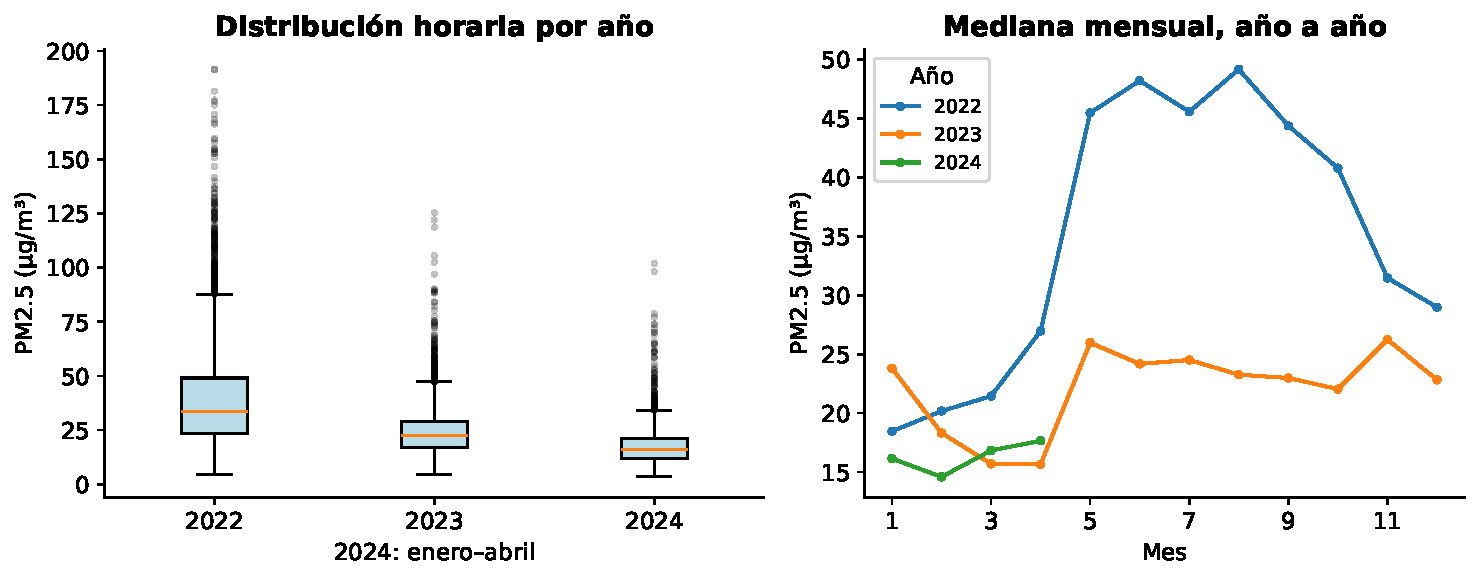
\includegraphics[width=\columnwidth]{figures/12_distribucion_anual.pdf}
\caption{Cambio de nivel entre años y comparación de medianas mensuales.}
\label{fig:regimen}
\end{figure}

\subsection{Dependencia temporal}
\label{sec:autocorrelacion}

Entre horas consecutivas la correlación de Pearson es de 0,912 (19.343 pares completos). La autocorrelación cae a 0,464 en el rezago 12 y vuelve a subir a 0,651 en el rezago 24, lo que muestra el ciclo diario. La autocorrelación parcial se concentra en el primer rezago (0,912), es negativa en el segundo ($-0{,}184$) y no supera 0,12 en valor absoluto entre los rezagos 3 y 24 (Fig.~\ref{fig:acf}). Los rezagos inmediatos aportan la información propia de corto plazo, mientras que el repunte a 24 horas corresponde al ciclo diario y puede representarse con variables de calendario en lugar de decenas de rezagos. Cuál de las dos opciones rinde más se responde comparando modelos con y sin calendario (pregunta de investigación 2).

\begin{figure}[t]
\centering
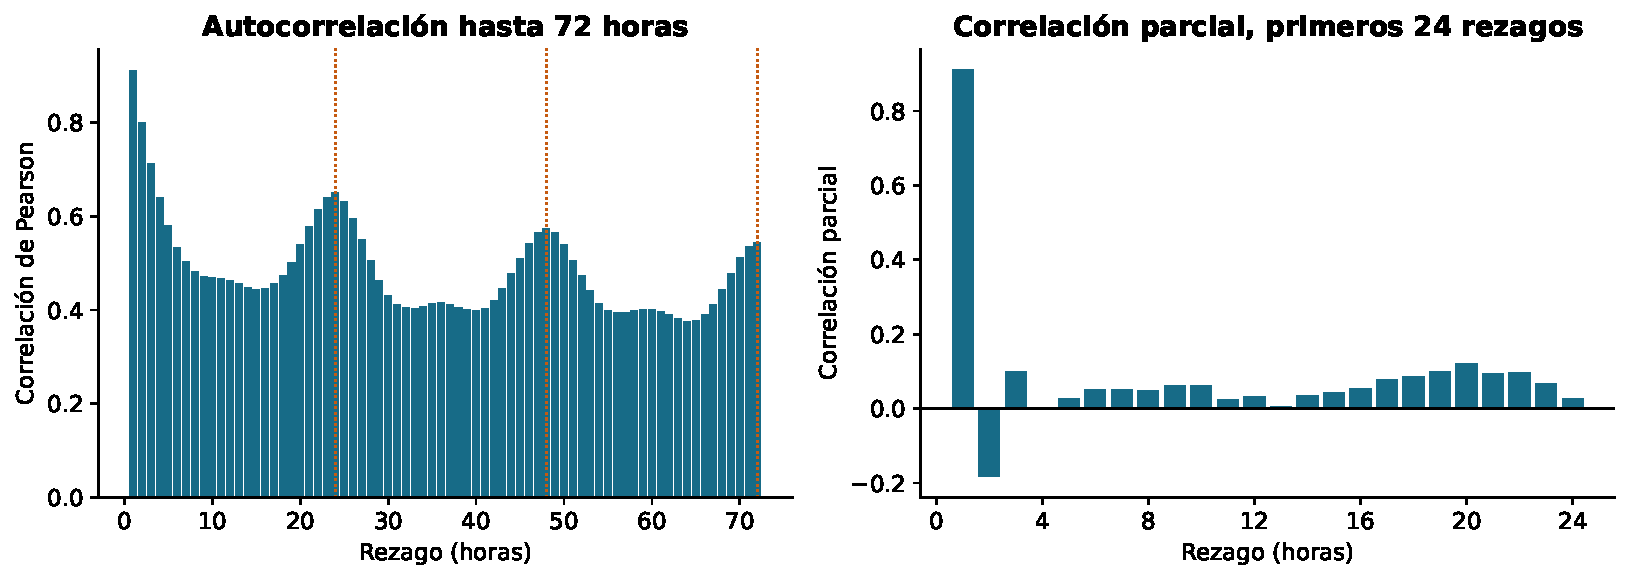
\includegraphics[width=\columnwidth]{figures/13_autocorrelacion.pdf}
\caption{Autocorrelación y autocorrelación parcial de PM2.5 hasta 48 horas, calculadas con las horas en que ambos valores están disponibles.}
\label{fig:acf}
\end{figure}

\subsection{Implicaciones para el modelado}
\label{sec:implicaciones}

El análisis exploratorio condiciona el diseño de la segunda etapa en cuatro puntos: los faltantes se agrupan en tramos y no se imputan, por lo que cada hora utilizable exige respuesta e historial completos; los valores extremos se conservan; la partición debe ser cronológica y sus métricas desagregadas por bloque, por el cambio de régimen; y el baseline natural es la persistencia, dada la correlación de 0,912 a una hora. Estas decisiones se concretan en la sección~\ref{sec:preproc}.
